\documentclass[twoside]{book}

% Packages required by doxygen
\usepackage{fixltx2e}
\usepackage{calc}
\usepackage{doxygen}
\usepackage{graphicx}
\usepackage[utf8]{inputenc}
\usepackage{makeidx}
\usepackage{multicol}
\usepackage{multirow}
\PassOptionsToPackage{warn}{textcomp}
\usepackage{textcomp}
\usepackage[nointegrals]{wasysym}
\usepackage[table]{xcolor}

% Font selection
\usepackage[T1]{fontenc}
\usepackage{mathptmx}
\usepackage[scaled=.90]{helvet}
\usepackage{courier}
\usepackage{amssymb}
\usepackage{sectsty}
\renewcommand{\familydefault}{\sfdefault}
\allsectionsfont{%
  \fontseries{bc}\selectfont%
  \color{darkgray}%
}
\renewcommand{\DoxyLabelFont}{%
  \fontseries{bc}\selectfont%
  \color{darkgray}%
}
\newcommand{\+}{\discretionary{\mbox{\scriptsize$\hookleftarrow$}}{}{}}

% Page & text layout
\usepackage{geometry}
\geometry{%
  a4paper,%
  top=2.5cm,%
  bottom=2.5cm,%
  left=2.5cm,%
  right=2.5cm%
}
\tolerance=750
\hfuzz=15pt
\hbadness=750
\setlength{\emergencystretch}{15pt}
\setlength{\parindent}{0cm}
\setlength{\parskip}{0.2cm}
\makeatletter
\renewcommand{\paragraph}{%
  \@startsection{paragraph}{4}{0ex}{-1.0ex}{1.0ex}{%
    \normalfont\normalsize\bfseries\SS@parafont%
  }%
}
\renewcommand{\subparagraph}{%
  \@startsection{subparagraph}{5}{0ex}{-1.0ex}{1.0ex}{%
    \normalfont\normalsize\bfseries\SS@subparafont%
  }%
}
\makeatother

% Headers & footers
\usepackage{fancyhdr}
\pagestyle{fancyplain}
\fancyhead[LE]{\fancyplain{}{\bfseries\thepage}}
\fancyhead[CE]{\fancyplain{}{}}
\fancyhead[RE]{\fancyplain{}{\bfseries\leftmark}}
\fancyhead[LO]{\fancyplain{}{\bfseries\rightmark}}
\fancyhead[CO]{\fancyplain{}{}}
\fancyhead[RO]{\fancyplain{}{\bfseries\thepage}}
\fancyfoot[LE]{\fancyplain{}{}}
\fancyfoot[CE]{\fancyplain{}{}}
\fancyfoot[RE]{\fancyplain{}{\bfseries\scriptsize Generated on Sun Nov 16 2014 16\+:36\+:59 for S\+O\+F\+T336 by Doxygen }}
\fancyfoot[LO]{\fancyplain{}{\bfseries\scriptsize Generated on Sun Nov 16 2014 16\+:36\+:59 for S\+O\+F\+T336 by Doxygen }}
\fancyfoot[CO]{\fancyplain{}{}}
\fancyfoot[RO]{\fancyplain{}{}}
\renewcommand{\footrulewidth}{0.4pt}
\renewcommand{\chaptermark}[1]{%
  \markboth{#1}{}%
}
\renewcommand{\sectionmark}[1]{%
  \markright{\thesection\ #1}%
}

% Indices & bibliography
\usepackage{natbib}
\usepackage[titles]{tocloft}
\setcounter{tocdepth}{3}
\setcounter{secnumdepth}{5}
\makeindex

% Hyperlinks (required, but should be loaded last)
\usepackage{ifpdf}
\ifpdf
  \usepackage[pdftex,pagebackref=true]{hyperref}
\else
  \usepackage[ps2pdf,pagebackref=true]{hyperref}
\fi
\hypersetup{%
  colorlinks=true,%
  linkcolor=blue,%
  citecolor=blue,%
  unicode%
}

% Custom commands
\newcommand{\clearemptydoublepage}{%
  \newpage{\pagestyle{empty}\cleardoublepage}%
}


%===== C O N T E N T S =====

\begin{document}

% Titlepage & ToC
\hypersetup{pageanchor=false,
             bookmarks=true,
             bookmarksnumbered=true,
             pdfencoding=unicode
            }
\pagenumbering{roman}
\begin{titlepage}
\vspace*{7cm}
\begin{center}%
{\Large S\+O\+F\+T336 \\[1ex]\large 1.\+0 }\\
\vspace*{1cm}
{\large Generated by Doxygen 1.8.8}\\
\vspace*{0.5cm}
{\small Sun Nov 16 2014 16:36:59}\\
\end{center}
\end{titlepage}
\clearemptydoublepage
\tableofcontents
\clearemptydoublepage
\pagenumbering{arabic}
\hypersetup{pageanchor=true}

%--- Begin generated contents ---
\chapter{test}
\label{index}\hypertarget{index}{}The program is a simple Vo\+I\+P application that is cross-\/platform and allows users to “conference call” across a local network. Transmission is near instant (dependant on network performance), and there is no noticeable lag or latency when communicating. It allows participants to select whether they wish to broadcast or listen (or both). Audio is compressed using zlib, and is sent at C\+D quality (44.\+1khz, 16 channels), and does not utilise any audio codecs. 
\chapter{Hierarchical Index}
\section{Class Hierarchy}
This inheritance list is sorted roughly, but not completely, alphabetically\+:\begin{DoxyCompactList}
\item Q\+Abstract\+Table\+Model\begin{DoxyCompactList}
\item \contentsline{section}{Client\+List}{\pageref{class_client_list}}{}
\end{DoxyCompactList}
\item Q\+Main\+Window\begin{DoxyCompactList}
\item \contentsline{section}{Main\+Window}{\pageref{class_main_window}}{}
\end{DoxyCompactList}
\item Q\+Object\begin{DoxyCompactList}
\item \contentsline{section}{Audio\+Input}{\pageref{class_audio_input}}{}
\item \contentsline{section}{Audio\+Output}{\pageref{class_audio_output}}{}
\item \contentsline{section}{Client}{\pageref{class_client}}{}
\item \contentsline{section}{Client\+Info}{\pageref{class_client_info}}{}
\item \contentsline{section}{Server}{\pageref{class_server}}{}
\end{DoxyCompactList}
\end{DoxyCompactList}

\chapter{Class Index}
\section{Class List}
Here are the classes, structs, unions and interfaces with brief descriptions\+:\begin{DoxyCompactList}
\item\contentsline{section}{\hyperlink{class_audio_input}{Audio\+Input} \\*The \hyperlink{class_audio_input}{Audio\+Input} class, interface/controller for the audio input device }{\pageref{class_audio_input}}{}
\item\contentsline{section}{\hyperlink{class_audio_output}{Audio\+Output} \\*The \hyperlink{class_audio_output}{Audio\+Output} class, interface/controller for audio output device }{\pageref{class_audio_output}}{}
\item\contentsline{section}{\hyperlink{class_client}{Client} \\*The \hyperlink{class_client}{Client} class, responsible for reading and processing datagrams, and playing audio }{\pageref{class_client}}{}
\item\contentsline{section}{\hyperlink{class_client_info}{Client\+Info} \\*The \hyperlink{class_client_info}{Client\+Info} class, holds client I\+P address, and a timeout timer }{\pageref{class_client_info}}{}
\item\contentsline{section}{\hyperlink{class_client_list}{Client\+List} \\*The \hyperlink{class_client_list}{Client\+List} class, holds a Q\+List of \hyperlink{class_client_info}{Client\+Info}, which is used to store network clients }{\pageref{class_client_list}}{}
\item\contentsline{section}{\hyperlink{class_main_window}{Main\+Window} \\*The \hyperlink{class_main_window}{Main\+Window} class, view for the application }{\pageref{class_main_window}}{}
\item\contentsline{section}{\hyperlink{class_server}{Server} \\*The \hyperlink{class_server}{Server} class, responsible for reading from the audio device and sending across the network, and sending broadcast information }{\pageref{class_server}}{}
\end{DoxyCompactList}

\chapter{Class Documentation}
\hypertarget{class_audio_input}{\section{Audio\+Input Class Reference}
\label{class_audio_input}\index{Audio\+Input@{Audio\+Input}}
}


The \hyperlink{class_audio_input}{Audio\+Input} class, interface/controller for the audio input device.  




{\ttfamily \#include $<$audioinput.\+h$>$}

Inheritance diagram for Audio\+Input\+:\begin{figure}[H]
\begin{center}
\leavevmode
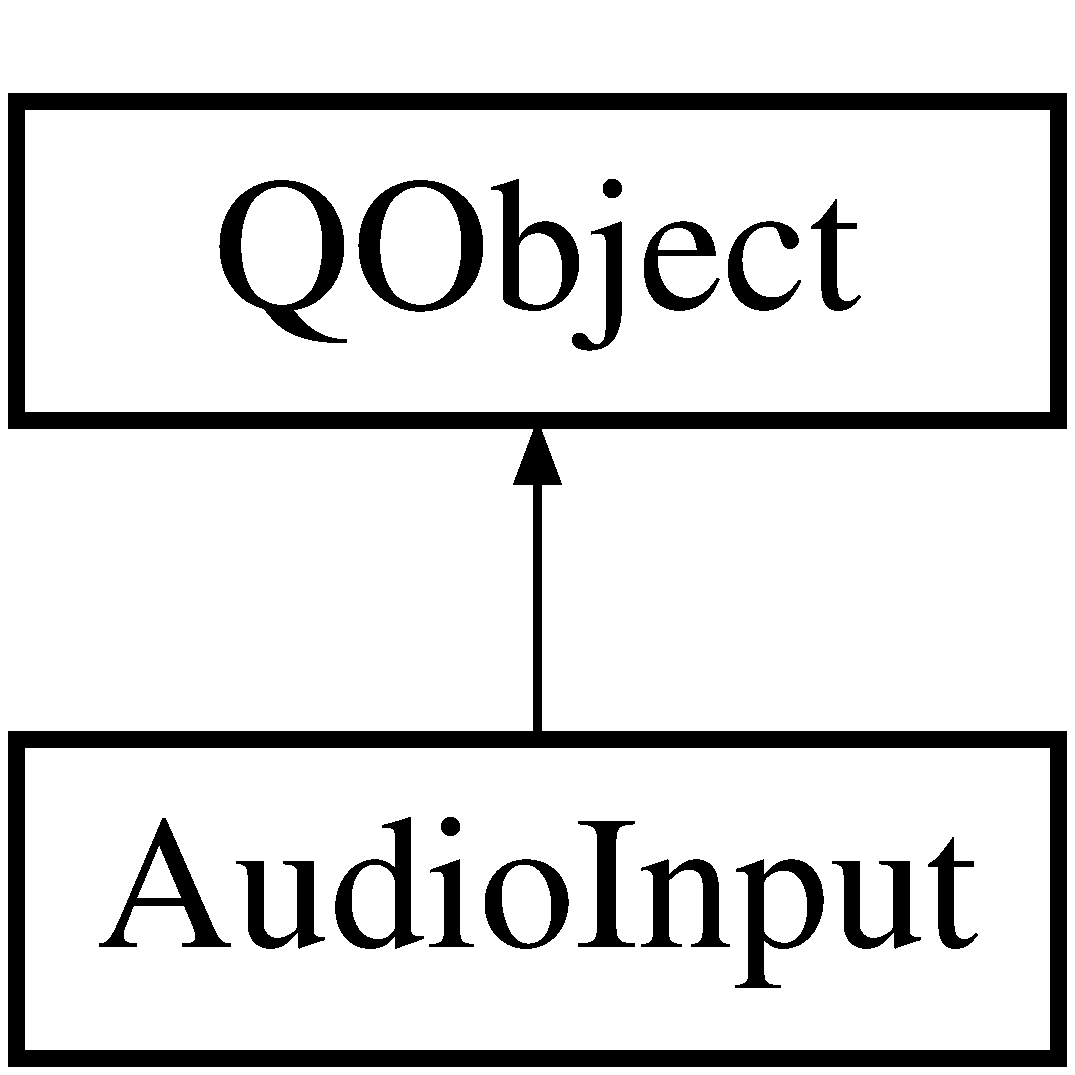
\includegraphics[height=2.000000cm]{class_audio_input}
\end{center}
\end{figure}
\subsection*{Signals}
\begin{DoxyCompactItemize}
\item 
\hypertarget{class_audio_input_a145b9998b45bf913ded725f47f9dfdf2}{void {\bfseries data\+Ready} (Q\+Byte\+Array data)}\label{class_audio_input_a145b9998b45bf913ded725f47f9dfdf2}

\end{DoxyCompactItemize}
\subsection*{Public Member Functions}
\begin{DoxyCompactItemize}
\item 
\hyperlink{class_audio_input_a49f4a3466e987468f1f94bed64e29fa9}{Audio\+Input} (Q\+Audio\+Device\+Info devinfo, Q\+Object $\ast$parent=0)
\begin{DoxyCompactList}\small\item\em \hyperlink{class_audio_input_a49f4a3466e987468f1f94bed64e29fa9}{Audio\+Input\+::\+Audio\+Input} default constructor for the \hyperlink{class_audio_input}{Audio\+Input}. \end{DoxyCompactList}\item 
void \hyperlink{class_audio_input_a52f68fb48010592d01166906b2961e21}{change\+Device} (Q\+Audio\+Device\+Info devinfo)
\begin{DoxyCompactList}\small\item\em \hyperlink{class_audio_input_a52f68fb48010592d01166906b2961e21}{Audio\+Input\+::change\+Device} changes the input audio device. \end{DoxyCompactList}\item 
void \hyperlink{class_audio_input_ad8bc7b12ac3476c85be6b19a8c4f9330}{start\+Device} (Q\+Audio\+Device\+Info devinfo)
\begin{DoxyCompactList}\small\item\em \hyperlink{class_audio_input_ad8bc7b12ac3476c85be6b19a8c4f9330}{Audio\+Input\+::start\+Device} initialises the audio and starts recording. \end{DoxyCompactList}\item 
void \hyperlink{class_audio_input_a268775cff2a682024a5d68308aa909c2}{set\+Volume} (float volume)
\begin{DoxyCompactList}\small\item\em \hyperlink{class_audio_input_a268775cff2a682024a5d68308aa909c2}{Audio\+Input\+::set\+Volume} sets input volume of device. \end{DoxyCompactList}\item 
\hypertarget{class_audio_input_a28aecfc4dc6d576674ee1b923c3d6f24}{void \hyperlink{class_audio_input_a28aecfc4dc6d576674ee1b923c3d6f24}{start\+Audio} ()}\label{class_audio_input_a28aecfc4dc6d576674ee1b923c3d6f24}

\begin{DoxyCompactList}\small\item\em \hyperlink{class_audio_input_a28aecfc4dc6d576674ee1b923c3d6f24}{Audio\+Input\+::start\+Audio} sets send\+Audio to true; starts sending audio. \end{DoxyCompactList}\item 
\hypertarget{class_audio_input_a90062672a92bb9250de567e1746913c7}{void \hyperlink{class_audio_input_a90062672a92bb9250de567e1746913c7}{stop\+Audio} ()}\label{class_audio_input_a90062672a92bb9250de567e1746913c7}

\begin{DoxyCompactList}\small\item\em \hyperlink{class_audio_input_a90062672a92bb9250de567e1746913c7}{Audio\+Input\+::stop\+Audio} sets send\+Audio to false; stops sending audio. \end{DoxyCompactList}\end{DoxyCompactItemize}
\subsection*{Private Slots}
\begin{DoxyCompactItemize}
\item 
\hypertarget{class_audio_input_adb78a37081a55c5187a1fe320ddd7266}{void \hyperlink{class_audio_input_adb78a37081a55c5187a1fe320ddd7266}{ready\+Read} ()}\label{class_audio_input_adb78a37081a55c5187a1fe320ddd7266}

\begin{DoxyCompactList}\small\item\em \hyperlink{class_audio_input_adb78a37081a55c5187a1fe320ddd7266}{Audio\+Input\+::ready\+Read} slot called when device is ready to read, emits data\+Ready() signal. \end{DoxyCompactList}\end{DoxyCompactItemize}
\subsection*{Private Attributes}
\begin{DoxyCompactItemize}
\item 
\hypertarget{class_audio_input_a51ba924ef3bdd93191890e76fe822e27}{Q\+Audio\+Input $\ast$ {\bfseries audio}}\label{class_audio_input_a51ba924ef3bdd93191890e76fe822e27}

\item 
\hypertarget{class_audio_input_a80188cedce4de076c4072b3c460fef6c}{Q\+I\+O\+Device $\ast$ {\bfseries device}}\label{class_audio_input_a80188cedce4de076c4072b3c460fef6c}

\item 
\hypertarget{class_audio_input_a05d2d3b1c013ae5e407b306ca4ffe43c}{Q\+Audio\+Format {\bfseries format}}\label{class_audio_input_a05d2d3b1c013ae5e407b306ca4ffe43c}

\item 
\hypertarget{class_audio_input_ad139df9556fcff32cfc42dfd8560e850}{bool {\bfseries send\+Audio}}\label{class_audio_input_ad139df9556fcff32cfc42dfd8560e850}

\end{DoxyCompactItemize}


\subsection{Detailed Description}
The \hyperlink{class_audio_input}{Audio\+Input} class, interface/controller for the audio input device. 

\subsection{Constructor \& Destructor Documentation}
\hypertarget{class_audio_input_a49f4a3466e987468f1f94bed64e29fa9}{\index{Audio\+Input@{Audio\+Input}!Audio\+Input@{Audio\+Input}}
\index{Audio\+Input@{Audio\+Input}!Audio\+Input@{Audio\+Input}}
\subsubsection[{Audio\+Input}]{\setlength{\rightskip}{0pt plus 5cm}Audio\+Input\+::\+Audio\+Input (
\begin{DoxyParamCaption}
\item[{Q\+Audio\+Device\+Info}]{devinfo, }
\item[{Q\+Object $\ast$}]{parent = {\ttfamily 0}}
\end{DoxyParamCaption}
)\hspace{0.3cm}{\ttfamily [explicit]}}}\label{class_audio_input_a49f4a3466e987468f1f94bed64e29fa9}


\hyperlink{class_audio_input_a49f4a3466e987468f1f94bed64e29fa9}{Audio\+Input\+::\+Audio\+Input} default constructor for the \hyperlink{class_audio_input}{Audio\+Input}. 


\begin{DoxyParams}{Parameters}
{\em devinfo} & the device info to use when initialiasing. \\
\hline
{\em parent} & the parent object. \\
\hline
\end{DoxyParams}


\subsection{Member Function Documentation}
\hypertarget{class_audio_input_a52f68fb48010592d01166906b2961e21}{\index{Audio\+Input@{Audio\+Input}!change\+Device@{change\+Device}}
\index{change\+Device@{change\+Device}!Audio\+Input@{Audio\+Input}}
\subsubsection[{change\+Device}]{\setlength{\rightskip}{0pt plus 5cm}void Audio\+Input\+::change\+Device (
\begin{DoxyParamCaption}
\item[{Q\+Audio\+Device\+Info}]{devinfo}
\end{DoxyParamCaption}
)}}\label{class_audio_input_a52f68fb48010592d01166906b2961e21}


\hyperlink{class_audio_input_a52f68fb48010592d01166906b2961e21}{Audio\+Input\+::change\+Device} changes the input audio device. 


\begin{DoxyParams}{Parameters}
{\em devinfo} & the new audio device. \\
\hline
\end{DoxyParams}
\hypertarget{class_audio_input_a268775cff2a682024a5d68308aa909c2}{\index{Audio\+Input@{Audio\+Input}!set\+Volume@{set\+Volume}}
\index{set\+Volume@{set\+Volume}!Audio\+Input@{Audio\+Input}}
\subsubsection[{set\+Volume}]{\setlength{\rightskip}{0pt plus 5cm}void Audio\+Input\+::set\+Volume (
\begin{DoxyParamCaption}
\item[{float}]{volume}
\end{DoxyParamCaption}
)}}\label{class_audio_input_a268775cff2a682024a5d68308aa909c2}


\hyperlink{class_audio_input_a268775cff2a682024a5d68308aa909c2}{Audio\+Input\+::set\+Volume} sets input volume of device. 


\begin{DoxyParams}{Parameters}
{\em volume} & the volume to set. \\
\hline
\end{DoxyParams}
\hypertarget{class_audio_input_ad8bc7b12ac3476c85be6b19a8c4f9330}{\index{Audio\+Input@{Audio\+Input}!start\+Device@{start\+Device}}
\index{start\+Device@{start\+Device}!Audio\+Input@{Audio\+Input}}
\subsubsection[{start\+Device}]{\setlength{\rightskip}{0pt plus 5cm}void Audio\+Input\+::start\+Device (
\begin{DoxyParamCaption}
\item[{Q\+Audio\+Device\+Info}]{devinfo}
\end{DoxyParamCaption}
)}}\label{class_audio_input_ad8bc7b12ac3476c85be6b19a8c4f9330}


\hyperlink{class_audio_input_ad8bc7b12ac3476c85be6b19a8c4f9330}{Audio\+Input\+::start\+Device} initialises the audio and starts recording. 


\begin{DoxyParams}{Parameters}
{\em devinfo} & device to read from. \\
\hline
\end{DoxyParams}


The documentation for this class was generated from the following files\+:\begin{DoxyCompactItemize}
\item 
soft336/audioinput.\+h\item 
soft336/audioinput.\+cpp\end{DoxyCompactItemize}

\hypertarget{class_audio_output}{\section{Audio\+Output Class Reference}
\label{class_audio_output}\index{Audio\+Output@{Audio\+Output}}
}


The \hyperlink{class_audio_output}{Audio\+Output} class, interface/controller for audio output device.  




{\ttfamily \#include $<$audiooutput.\+h$>$}

Inheritance diagram for Audio\+Output\+:\begin{figure}[H]
\begin{center}
\leavevmode
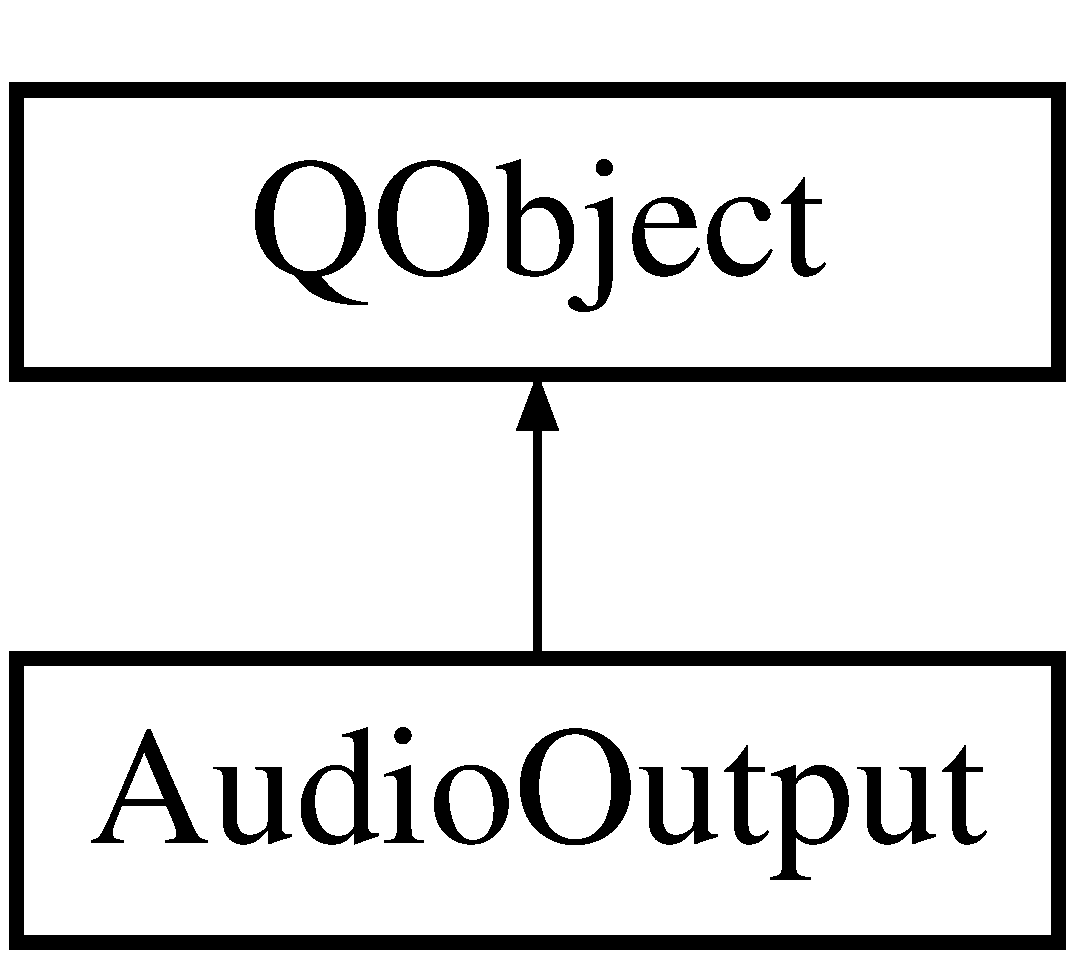
\includegraphics[height=2.000000cm]{class_audio_output}
\end{center}
\end{figure}
\subsection*{Public Slots}
\begin{DoxyCompactItemize}
\item 
void \hyperlink{class_audio_output_a7daeee7334313b255eac6b2d31e54729}{write\+Data} (Q\+Byte\+Array data)
\begin{DoxyCompactList}\small\item\em \hyperlink{class_audio_output_a7daeee7334313b255eac6b2d31e54729}{Audio\+Output\+::write\+Data} writes data to the output. \end{DoxyCompactList}\end{DoxyCompactItemize}
\subsection*{Public Member Functions}
\begin{DoxyCompactItemize}
\item 
\hyperlink{class_audio_output_a1536f8f50eb732249ffbcf491b04dee2}{Audio\+Output} (Q\+Object $\ast$parent=0)
\begin{DoxyCompactList}\small\item\em \hyperlink{class_audio_output_a1536f8f50eb732249ffbcf491b04dee2}{Audio\+Output\+::\+Audio\+Output} default constructor for \hyperlink{class_audio_input}{Audio\+Input}. \end{DoxyCompactList}\item 
void \hyperlink{class_audio_output_a97008d6a17c3dc03c64e421f563e04b8}{set\+Volume} (float volume)
\begin{DoxyCompactList}\small\item\em \hyperlink{class_audio_output_a97008d6a17c3dc03c64e421f563e04b8}{Audio\+Output\+::set\+Volume} set the volume of the output device. \end{DoxyCompactList}\end{DoxyCompactItemize}
\subsection*{Private Attributes}
\begin{DoxyCompactItemize}
\item 
\hypertarget{class_audio_output_a4503e92a56cb81ff0fe356c979c86189}{Q\+Audio\+Output $\ast$ {\bfseries audio}}\label{class_audio_output_a4503e92a56cb81ff0fe356c979c86189}

\item 
\hypertarget{class_audio_output_a97cd665e8a886d9e46cadd77168077cd}{Q\+I\+O\+Device $\ast$ {\bfseries device}}\label{class_audio_output_a97cd665e8a886d9e46cadd77168077cd}

\end{DoxyCompactItemize}


\subsection{Detailed Description}
The \hyperlink{class_audio_output}{Audio\+Output} class, interface/controller for audio output device. 

\subsection{Constructor \& Destructor Documentation}
\hypertarget{class_audio_output_a1536f8f50eb732249ffbcf491b04dee2}{\index{Audio\+Output@{Audio\+Output}!Audio\+Output@{Audio\+Output}}
\index{Audio\+Output@{Audio\+Output}!Audio\+Output@{Audio\+Output}}
\subsubsection[{Audio\+Output}]{\setlength{\rightskip}{0pt plus 5cm}Audio\+Output\+::\+Audio\+Output (
\begin{DoxyParamCaption}
\item[{Q\+Object $\ast$}]{parent = {\ttfamily 0}}
\end{DoxyParamCaption}
)\hspace{0.3cm}{\ttfamily [explicit]}}}\label{class_audio_output_a1536f8f50eb732249ffbcf491b04dee2}


\hyperlink{class_audio_output_a1536f8f50eb732249ffbcf491b04dee2}{Audio\+Output\+::\+Audio\+Output} default constructor for \hyperlink{class_audio_input}{Audio\+Input}. 


\begin{DoxyParams}{Parameters}
{\em parent} & the parent object. \\
\hline
\end{DoxyParams}


\subsection{Member Function Documentation}
\hypertarget{class_audio_output_a97008d6a17c3dc03c64e421f563e04b8}{\index{Audio\+Output@{Audio\+Output}!set\+Volume@{set\+Volume}}
\index{set\+Volume@{set\+Volume}!Audio\+Output@{Audio\+Output}}
\subsubsection[{set\+Volume}]{\setlength{\rightskip}{0pt plus 5cm}void Audio\+Output\+::set\+Volume (
\begin{DoxyParamCaption}
\item[{float}]{volume}
\end{DoxyParamCaption}
)}}\label{class_audio_output_a97008d6a17c3dc03c64e421f563e04b8}


\hyperlink{class_audio_output_a97008d6a17c3dc03c64e421f563e04b8}{Audio\+Output\+::set\+Volume} set the volume of the output device. 


\begin{DoxyParams}{Parameters}
{\em volume} & the volume to set. \\
\hline
\end{DoxyParams}
\hypertarget{class_audio_output_a7daeee7334313b255eac6b2d31e54729}{\index{Audio\+Output@{Audio\+Output}!write\+Data@{write\+Data}}
\index{write\+Data@{write\+Data}!Audio\+Output@{Audio\+Output}}
\subsubsection[{write\+Data}]{\setlength{\rightskip}{0pt plus 5cm}void Audio\+Output\+::write\+Data (
\begin{DoxyParamCaption}
\item[{Q\+Byte\+Array}]{data}
\end{DoxyParamCaption}
)\hspace{0.3cm}{\ttfamily [slot]}}}\label{class_audio_output_a7daeee7334313b255eac6b2d31e54729}


\hyperlink{class_audio_output_a7daeee7334313b255eac6b2d31e54729}{Audio\+Output\+::write\+Data} writes data to the output. 


\begin{DoxyParams}{Parameters}
{\em data} & the data to write. \\
\hline
\end{DoxyParams}


The documentation for this class was generated from the following files\+:\begin{DoxyCompactItemize}
\item 
soft336/audiooutput.\+h\item 
soft336/audiooutput.\+cpp\end{DoxyCompactItemize}

\hypertarget{class_client}{\section{Client Class Reference}
\label{class_client}\index{Client@{Client}}
}


The \hyperlink{class_client}{Client} class, responsible for reading and processing datagrams, and playing audio.  




{\ttfamily \#include $<$client.\+h$>$}

Inheritance diagram for Client\+:\begin{figure}[H]
\begin{center}
\leavevmode
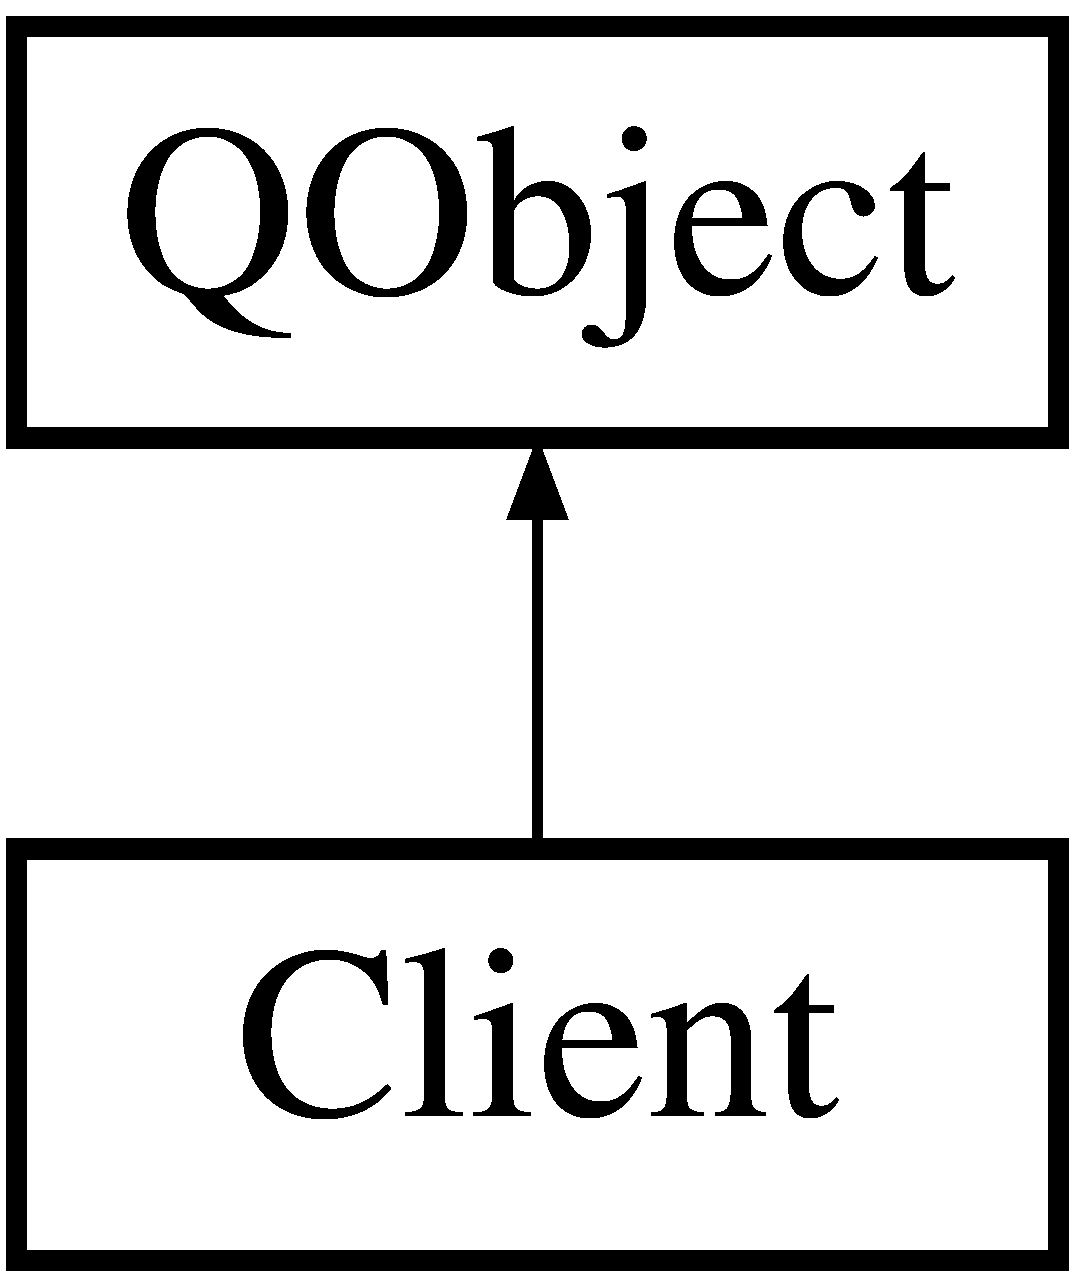
\includegraphics[height=2.000000cm]{class_client}
\end{center}
\end{figure}
\subsection*{Signals}
\begin{DoxyCompactItemize}
\item 
\hypertarget{class_client_a988a44e569be731da0d7186afa965b7c}{void {\bfseries client\+Broadcast\+Received} (Q\+String client\+Address, Q\+String control\+String)}\label{class_client_a988a44e569be731da0d7186afa965b7c}

\end{DoxyCompactItemize}
\subsection*{Public Member Functions}
\begin{DoxyCompactItemize}
\item 
\hyperlink{class_client_a7832757f3fa37f564a21cb2b79b2baad}{Client} (Q\+Object $\ast$parent=0)
\begin{DoxyCompactList}\small\item\em \hyperlink{class_client_a7832757f3fa37f564a21cb2b79b2baad}{Client\+::\+Client} Default constructor for client. \end{DoxyCompactList}\item 
\hypertarget{class_client_a82ad726820ceb6332a603ea075c39105}{void \hyperlink{class_client_a82ad726820ceb6332a603ea075c39105}{start\+Listen} ()}\label{class_client_a82ad726820ceb6332a603ea075c39105}

\begin{DoxyCompactList}\small\item\em \hyperlink{class_client_a82ad726820ceb6332a603ea075c39105}{Client\+::start\+Listen} sets listen bool to true; starts writing audio to the device. \end{DoxyCompactList}\item 
\hypertarget{class_client_ad29f4f2cf64ca25ec2f7d092e6c9fd07}{void \hyperlink{class_client_ad29f4f2cf64ca25ec2f7d092e6c9fd07}{end\+Listen} ()}\label{class_client_ad29f4f2cf64ca25ec2f7d092e6c9fd07}

\begin{DoxyCompactList}\small\item\em \hyperlink{class_client_ad29f4f2cf64ca25ec2f7d092e6c9fd07}{Client\+::end\+Listen} sets listen bool to false; stops writing audio to the device. \end{DoxyCompactList}\item 
void \hyperlink{class_client_a1ff8c64a0e2e9563c7728990b16f720c}{set\+Volume} (float volume)
\begin{DoxyCompactList}\small\item\em \hyperlink{class_client_a1ff8c64a0e2e9563c7728990b16f720c}{Client\+::set\+Volume} sets the volume of the device. \end{DoxyCompactList}\end{DoxyCompactItemize}
\subsection*{Private Slots}
\begin{DoxyCompactItemize}
\item 
\hypertarget{class_client_abca3b984bee88e07ef8f81046e7398a9}{void \hyperlink{class_client_abca3b984bee88e07ef8f81046e7398a9}{read\+Datagrams} ()}\label{class_client_abca3b984bee88e07ef8f81046e7398a9}

\begin{DoxyCompactList}\small\item\em \hyperlink{class_client_abca3b984bee88e07ef8f81046e7398a9}{Client\+::read\+Datagrams} reads datagrams from the socket. \end{DoxyCompactList}\end{DoxyCompactItemize}
\subsection*{Private Attributes}
\begin{DoxyCompactItemize}
\item 
\hypertarget{class_client_a4e56fbe8e9ba4b17a676a64353bf80e0}{\hyperlink{class_audio_output}{Audio\+Output} $\ast$ {\bfseries output}}\label{class_client_a4e56fbe8e9ba4b17a676a64353bf80e0}

\item 
\hypertarget{class_client_ac8198ee0a28bc42b46996c0188743631}{Q\+Udp\+Socket $\ast$ {\bfseries socket}}\label{class_client_ac8198ee0a28bc42b46996c0188743631}

\item 
\hypertarget{class_client_a073d7935e0e7be937513d86c150d2d7c}{bool {\bfseries listen}}\label{class_client_a073d7935e0e7be937513d86c150d2d7c}

\end{DoxyCompactItemize}


\subsection{Detailed Description}
The \hyperlink{class_client}{Client} class, responsible for reading and processing datagrams, and playing audio. 

\subsection{Constructor \& Destructor Documentation}
\hypertarget{class_client_a7832757f3fa37f564a21cb2b79b2baad}{\index{Client@{Client}!Client@{Client}}
\index{Client@{Client}!Client@{Client}}
\subsubsection[{Client}]{\setlength{\rightskip}{0pt plus 5cm}Client\+::\+Client (
\begin{DoxyParamCaption}
\item[{Q\+Object $\ast$}]{parent = {\ttfamily 0}}
\end{DoxyParamCaption}
)\hspace{0.3cm}{\ttfamily [explicit]}}}\label{class_client_a7832757f3fa37f564a21cb2b79b2baad}


\hyperlink{class_client_a7832757f3fa37f564a21cb2b79b2baad}{Client\+::\+Client} Default constructor for client. 


\begin{DoxyParams}{Parameters}
{\em parent} & the Parent Object \\
\hline
\end{DoxyParams}


\subsection{Member Function Documentation}
\hypertarget{class_client_a1ff8c64a0e2e9563c7728990b16f720c}{\index{Client@{Client}!set\+Volume@{set\+Volume}}
\index{set\+Volume@{set\+Volume}!Client@{Client}}
\subsubsection[{set\+Volume}]{\setlength{\rightskip}{0pt plus 5cm}void Client\+::set\+Volume (
\begin{DoxyParamCaption}
\item[{float}]{volume}
\end{DoxyParamCaption}
)}}\label{class_client_a1ff8c64a0e2e9563c7728990b16f720c}


\hyperlink{class_client_a1ff8c64a0e2e9563c7728990b16f720c}{Client\+::set\+Volume} sets the volume of the device. 


\begin{DoxyParams}{Parameters}
{\em volume} & the volume to set. \\
\hline
\end{DoxyParams}


The documentation for this class was generated from the following files\+:\begin{DoxyCompactItemize}
\item 
client.\+h\item 
client.\+cpp\end{DoxyCompactItemize}

\hypertarget{class_client_info}{\section{Client\+Info Class Reference}
\label{class_client_info}\index{Client\+Info@{Client\+Info}}
}


The \hyperlink{class_client_info}{Client\+Info} class, holds client I\+P address, and a timeout timer.  




{\ttfamily \#include $<$model.\+h$>$}

Inheritance diagram for Client\+Info\+:\begin{figure}[H]
\begin{center}
\leavevmode
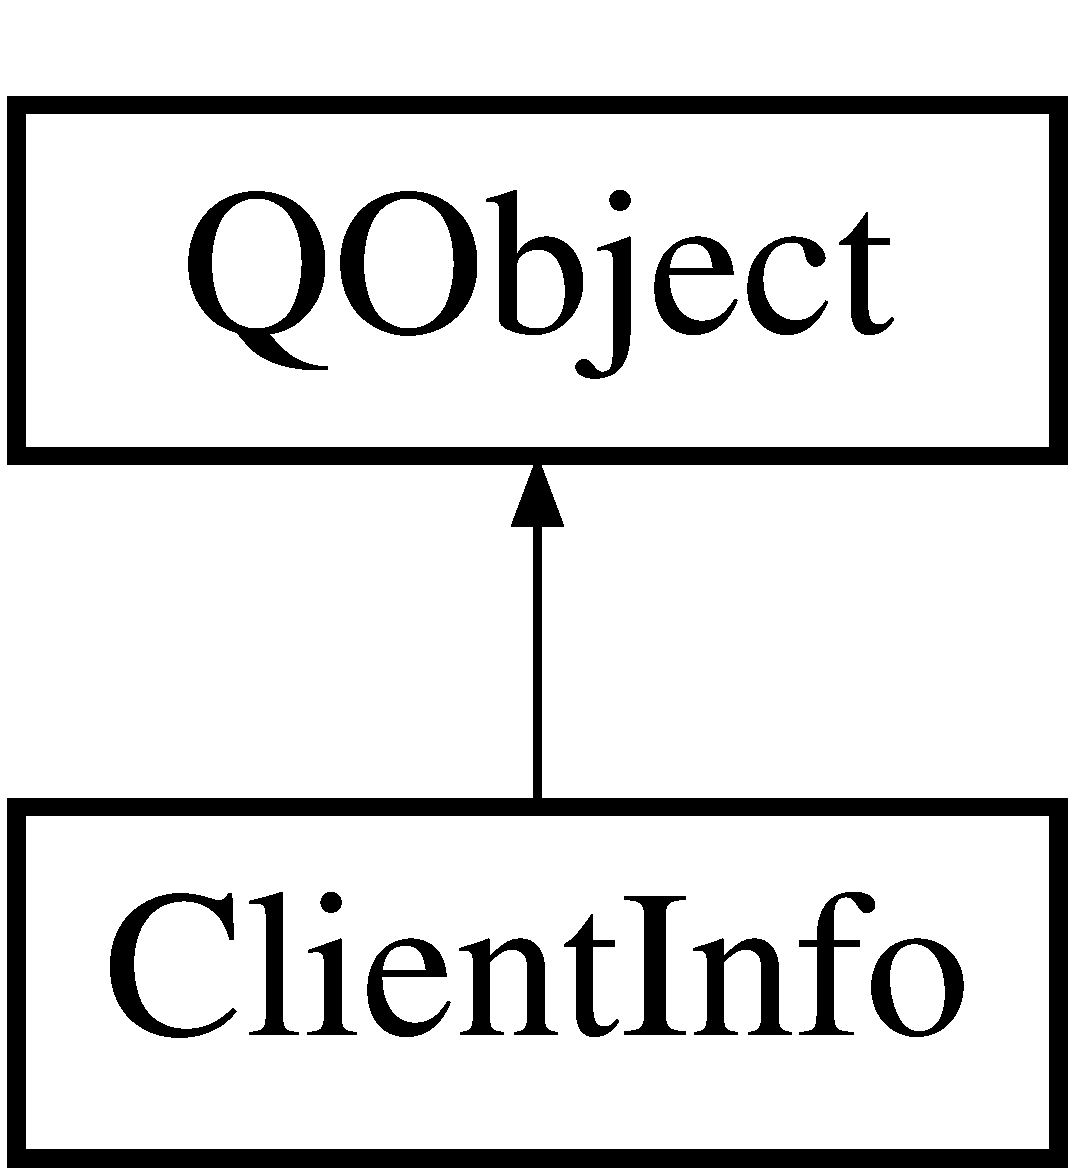
\includegraphics[height=2.000000cm]{class_client_info}
\end{center}
\end{figure}
\subsection*{Signals}
\begin{DoxyCompactItemize}
\item 
\hypertarget{class_client_info_a2c4800d43a301e2735b468a7a77f8932}{void {\bfseries client\+Timeout} (Q\+String c\+Address)}\label{class_client_info_a2c4800d43a301e2735b468a7a77f8932}

\end{DoxyCompactItemize}
\subsection*{Public Member Functions}
\begin{DoxyCompactItemize}
\item 
\hyperlink{class_client_info_a11c68fac6d389a2ad23fcb38452414d3}{Client\+Info} (Q\+Object $\ast$parent, Q\+String client\+Address)
\begin{DoxyCompactList}\small\item\em \hyperlink{class_client_info_a11c68fac6d389a2ad23fcb38452414d3}{Client\+Info\+::\+Client\+Info} default constructor for \hyperlink{class_client_info}{Client\+Info}. \end{DoxyCompactList}\item 
\hypertarget{class_client_info_a8dd4595978e5ff522b265f8b69dda437}{void \hyperlink{class_client_info_a8dd4595978e5ff522b265f8b69dda437}{restart\+Timer} ()}\label{class_client_info_a8dd4595978e5ff522b265f8b69dda437}

\begin{DoxyCompactList}\small\item\em \hyperlink{class_client_info_a8dd4595978e5ff522b265f8b69dda437}{Client\+Info\+::restart\+Timer} restarts a timer for a client. \end{DoxyCompactList}\item 
Q\+String \hyperlink{class_client_info_af84ec371c9c598a9fb8aee80ff951644}{get\+Address} () const 
\begin{DoxyCompactList}\small\item\em \hyperlink{class_client_info_af84ec371c9c598a9fb8aee80ff951644}{Client\+Info\+::get\+Address} get a clients I\+P address. \end{DoxyCompactList}\end{DoxyCompactItemize}
\subsection*{Public Attributes}
\begin{DoxyCompactItemize}
\item 
\hypertarget{class_client_info_ac8f77925933a5106abde8bec8bf17ade}{bool {\bfseries is\+Listening}}\label{class_client_info_ac8f77925933a5106abde8bec8bf17ade}

\item 
\hypertarget{class_client_info_a0cc5a8085094d51b3b7225f39cea1ceb}{bool {\bfseries is\+Broadcasting}}\label{class_client_info_a0cc5a8085094d51b3b7225f39cea1ceb}

\end{DoxyCompactItemize}
\subsection*{Private Slots}
\begin{DoxyCompactItemize}
\item 
\hypertarget{class_client_info_ada8a34df7cdad6456e11499ba4d147e2}{void \hyperlink{class_client_info_ada8a34df7cdad6456e11499ba4d147e2}{timer\+Expired} ()}\label{class_client_info_ada8a34df7cdad6456e11499ba4d147e2}

\begin{DoxyCompactList}\small\item\em \hyperlink{class_client_info_ada8a34df7cdad6456e11499ba4d147e2}{Client\+Info\+::timer\+Expired} called when timeout timer expires, informs the model. \end{DoxyCompactList}\end{DoxyCompactItemize}
\subsection*{Private Attributes}
\begin{DoxyCompactItemize}
\item 
\hypertarget{class_client_info_adae644f06d9b9db0b24e0a95eba7988a}{Q\+Timer $\ast$ {\bfseries timer}}\label{class_client_info_adae644f06d9b9db0b24e0a95eba7988a}

\item 
\hypertarget{class_client_info_a9edb182997bc69d43600172d9679286a}{Q\+String {\bfseries address}}\label{class_client_info_a9edb182997bc69d43600172d9679286a}

\end{DoxyCompactItemize}


\subsection{Detailed Description}
The \hyperlink{class_client_info}{Client\+Info} class, holds client I\+P address, and a timeout timer. 

\subsection{Constructor \& Destructor Documentation}
\hypertarget{class_client_info_a11c68fac6d389a2ad23fcb38452414d3}{\index{Client\+Info@{Client\+Info}!Client\+Info@{Client\+Info}}
\index{Client\+Info@{Client\+Info}!Client\+Info@{Client\+Info}}
\subsubsection[{Client\+Info}]{\setlength{\rightskip}{0pt plus 5cm}Client\+Info\+::\+Client\+Info (
\begin{DoxyParamCaption}
\item[{Q\+Object $\ast$}]{parent, }
\item[{Q\+String}]{client\+Address}
\end{DoxyParamCaption}
)}}\label{class_client_info_a11c68fac6d389a2ad23fcb38452414d3}


\hyperlink{class_client_info_a11c68fac6d389a2ad23fcb38452414d3}{Client\+Info\+::\+Client\+Info} default constructor for \hyperlink{class_client_info}{Client\+Info}. 


\begin{DoxyParams}{Parameters}
{\em parent} & the parent object. \\
\hline
{\em client\+Address} & the client I\+P address. \\
\hline
\end{DoxyParams}


\subsection{Member Function Documentation}
\hypertarget{class_client_info_af84ec371c9c598a9fb8aee80ff951644}{\index{Client\+Info@{Client\+Info}!get\+Address@{get\+Address}}
\index{get\+Address@{get\+Address}!Client\+Info@{Client\+Info}}
\subsubsection[{get\+Address}]{\setlength{\rightskip}{0pt plus 5cm}Q\+String Client\+Info\+::get\+Address (
\begin{DoxyParamCaption}
{}
\end{DoxyParamCaption}
) const}}\label{class_client_info_af84ec371c9c598a9fb8aee80ff951644}


\hyperlink{class_client_info_af84ec371c9c598a9fb8aee80ff951644}{Client\+Info\+::get\+Address} get a clients I\+P address. 

\begin{DoxyReturn}{Returns}
string containing clients I\+P address 
\end{DoxyReturn}


The documentation for this class was generated from the following files\+:\begin{DoxyCompactItemize}
\item 
model.\+h\item 
model.\+cpp\end{DoxyCompactItemize}

\hypertarget{class_client_list}{\section{Client\+List Class Reference}
\label{class_client_list}\index{Client\+List@{Client\+List}}
}


The \hyperlink{class_client_list}{Client\+List} class, holds a Q\+List of \hyperlink{class_client_info}{Client\+Info}, which is used to store network clients.  




{\ttfamily \#include $<$model.\+h$>$}

Inheritance diagram for Client\+List\+:\begin{figure}[H]
\begin{center}
\leavevmode
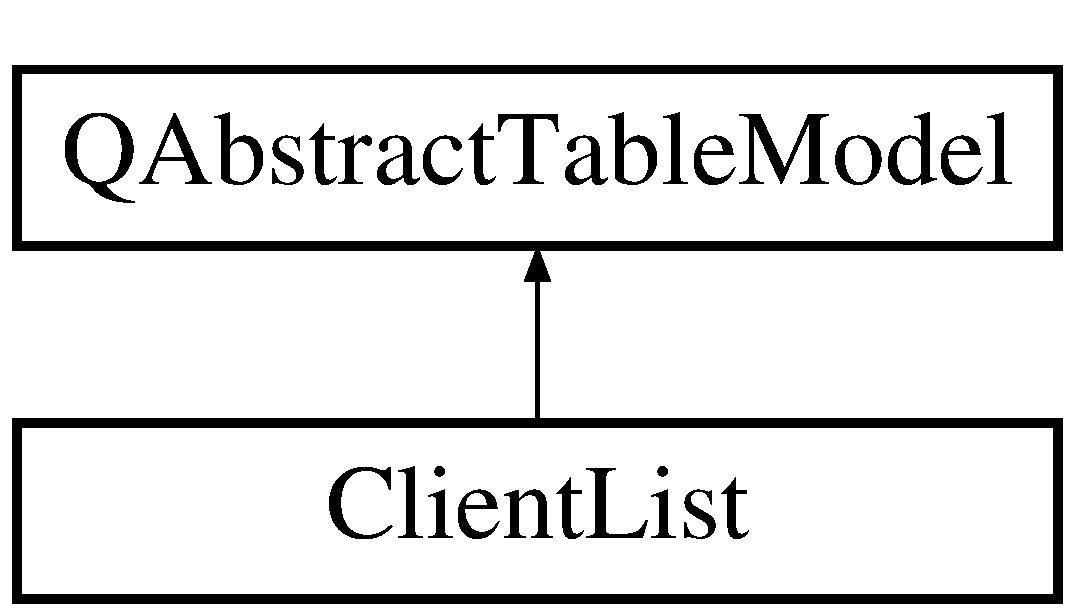
\includegraphics[height=2.000000cm]{class_client_list}
\end{center}
\end{figure}
\subsection*{Public Slots}
\begin{DoxyCompactItemize}
\item 
void \hyperlink{class_client_list_aa12147bebfba5ea2c293a816105eee13}{process\+Client} (Q\+String client\+Address, Q\+String control\+String)
\begin{DoxyCompactList}\small\item\em \hyperlink{class_client_list_aa12147bebfba5ea2c293a816105eee13}{Client\+List\+::process\+Client} process a client, adds them to the list if they don't exist, or updates an existing entry. \end{DoxyCompactList}\end{DoxyCompactItemize}
\subsection*{Public Member Functions}
\begin{DoxyCompactItemize}
\item 
\hyperlink{class_client_list_ad4f58e11ef5596e0dd71b868abca2cf6}{Client\+List} (Q\+Object $\ast$parent)
\begin{DoxyCompactList}\small\item\em \hyperlink{class_client_list_ad4f58e11ef5596e0dd71b868abca2cf6}{Client\+List\+::\+Client\+List} default constructor for \hyperlink{class_client_list}{Client\+List}. \end{DoxyCompactList}\item 
int \hyperlink{class_client_list_a306db79684b007b939da193370127a8d}{row\+Count} (const Q\+Model\+Index \&parent=Q\+Model\+Index()) const 
\begin{DoxyCompactList}\small\item\em \hyperlink{class_client_list_a306db79684b007b939da193370127a8d}{Client\+List\+::row\+Count} gets the size of the \hyperlink{class_client_list}{Client\+List}. \end{DoxyCompactList}\item 
int \hyperlink{class_client_list_a115194990c4699f46982aa53d6ca47d6}{column\+Count} (const Q\+Model\+Index \&parent) const 
\begin{DoxyCompactList}\small\item\em \hyperlink{class_client_list_a115194990c4699f46982aa53d6ca47d6}{Client\+List\+::column\+Count} returns amount of columns. \end{DoxyCompactList}\item 
Q\+Variant \hyperlink{class_client_list_aaa358efb8aad0f61194d56fe6735b4b6}{data} (const Q\+Model\+Index \&index, int role=Qt\+::\+Display\+Role) const 
\begin{DoxyCompactList}\small\item\em \hyperlink{class_client_list_aaa358efb8aad0f61194d56fe6735b4b6}{Client\+List\+::data} overloaded function for displaying the data in the table. \end{DoxyCompactList}\item 
Q\+Variant \hyperlink{class_client_list_ab63f37df0e3889d22224bddac30b4add}{header\+Data} (int section, Qt\+::\+Orientation orientation, int role) const 
\begin{DoxyCompactList}\small\item\em \hyperlink{class_client_list_ab63f37df0e3889d22224bddac30b4add}{Client\+List\+::header\+Data} overloaded function for setting the header columns in the table. \end{DoxyCompactList}\item 
Q\+Host\+Address \hyperlink{class_client_list_a78069b39dd0fa9d9af135d8e1538538a}{get\+Address\+At} (const Q\+Model\+Index \&index)
\begin{DoxyCompactList}\small\item\em \hyperlink{class_client_list_a78069b39dd0fa9d9af135d8e1538538a}{Client\+List\+::get\+Address\+At} returns a client address at the index specified. \end{DoxyCompactList}\item 
bool \hyperlink{class_client_list_a7a564d804ac940fe3364b0a5d54c03ce}{has\+Address} (Q\+String address)
\begin{DoxyCompactList}\small\item\em \hyperlink{class_client_list_a7a564d804ac940fe3364b0a5d54c03ce}{Client\+List\+::has\+Address} checks if the list contains the address, and if it does, restarts its timer. \end{DoxyCompactList}\end{DoxyCompactItemize}
\subsection*{Private Slots}
\begin{DoxyCompactItemize}
\item 
void \hyperlink{class_client_list_aac59ca6adda4d7e42c7d07e498bac7cd}{client\+Timeout} (Q\+String c\+Address)
\begin{DoxyCompactList}\small\item\em \hyperlink{class_client_list_aac59ca6adda4d7e42c7d07e498bac7cd}{Client\+List\+::client\+Timeout} called when a client timeouts. removes the client, and informs the view. \end{DoxyCompactList}\end{DoxyCompactItemize}
\subsection*{Private Attributes}
\begin{DoxyCompactItemize}
\item 
\hypertarget{class_client_list_a37fc232f71c36ccc9e36e30968f113a4}{Q\+List$<$ \hyperlink{class_client_info}{Client\+Info} $\ast$ $>$ {\bfseries clients}}\label{class_client_list_a37fc232f71c36ccc9e36e30968f113a4}

\end{DoxyCompactItemize}


\subsection{Detailed Description}
The \hyperlink{class_client_list}{Client\+List} class, holds a Q\+List of \hyperlink{class_client_info}{Client\+Info}, which is used to store network clients. 

\subsection{Constructor \& Destructor Documentation}
\hypertarget{class_client_list_ad4f58e11ef5596e0dd71b868abca2cf6}{\index{Client\+List@{Client\+List}!Client\+List@{Client\+List}}
\index{Client\+List@{Client\+List}!Client\+List@{Client\+List}}
\subsubsection[{Client\+List}]{\setlength{\rightskip}{0pt plus 5cm}Client\+List\+::\+Client\+List (
\begin{DoxyParamCaption}
\item[{Q\+Object $\ast$}]{parent}
\end{DoxyParamCaption}
)}}\label{class_client_list_ad4f58e11ef5596e0dd71b868abca2cf6}


\hyperlink{class_client_list_ad4f58e11ef5596e0dd71b868abca2cf6}{Client\+List\+::\+Client\+List} default constructor for \hyperlink{class_client_list}{Client\+List}. 


\begin{DoxyParams}{Parameters}
{\em parent} & the parent object. \\
\hline
\end{DoxyParams}


\subsection{Member Function Documentation}
\hypertarget{class_client_list_aac59ca6adda4d7e42c7d07e498bac7cd}{\index{Client\+List@{Client\+List}!client\+Timeout@{client\+Timeout}}
\index{client\+Timeout@{client\+Timeout}!Client\+List@{Client\+List}}
\subsubsection[{client\+Timeout}]{\setlength{\rightskip}{0pt plus 5cm}void Client\+List\+::client\+Timeout (
\begin{DoxyParamCaption}
\item[{Q\+String}]{address}
\end{DoxyParamCaption}
)\hspace{0.3cm}{\ttfamily [private]}, {\ttfamily [slot]}}}\label{class_client_list_aac59ca6adda4d7e42c7d07e498bac7cd}


\hyperlink{class_client_list_aac59ca6adda4d7e42c7d07e498bac7cd}{Client\+List\+::client\+Timeout} called when a client timeouts. removes the client, and informs the view. 


\begin{DoxyParams}{Parameters}
{\em address} & \\
\hline
\end{DoxyParams}
\hypertarget{class_client_list_a115194990c4699f46982aa53d6ca47d6}{\index{Client\+List@{Client\+List}!column\+Count@{column\+Count}}
\index{column\+Count@{column\+Count}!Client\+List@{Client\+List}}
\subsubsection[{column\+Count}]{\setlength{\rightskip}{0pt plus 5cm}int Client\+List\+::column\+Count (
\begin{DoxyParamCaption}
\item[{const Q\+Model\+Index \&}]{parent}
\end{DoxyParamCaption}
) const}}\label{class_client_list_a115194990c4699f46982aa53d6ca47d6}


\hyperlink{class_client_list_a115194990c4699f46982aa53d6ca47d6}{Client\+List\+::column\+Count} returns amount of columns. 

\begin{DoxyReturn}{Returns}
int of the number of columns. 
\end{DoxyReturn}
\hypertarget{class_client_list_aaa358efb8aad0f61194d56fe6735b4b6}{\index{Client\+List@{Client\+List}!data@{data}}
\index{data@{data}!Client\+List@{Client\+List}}
\subsubsection[{data}]{\setlength{\rightskip}{0pt plus 5cm}Q\+Variant Client\+List\+::data (
\begin{DoxyParamCaption}
\item[{const Q\+Model\+Index \&}]{index, }
\item[{int}]{role = {\ttfamily Qt\+:\+:DisplayRole}}
\end{DoxyParamCaption}
) const}}\label{class_client_list_aaa358efb8aad0f61194d56fe6735b4b6}


\hyperlink{class_client_list_aaa358efb8aad0f61194d56fe6735b4b6}{Client\+List\+::data} overloaded function for displaying the data in the table. 


\begin{DoxyParams}{Parameters}
{\em index} & \\
\hline
{\em role} & \\
\hline
\end{DoxyParams}
\begin{DoxyReturn}{Returns}

\end{DoxyReturn}
\hypertarget{class_client_list_a78069b39dd0fa9d9af135d8e1538538a}{\index{Client\+List@{Client\+List}!get\+Address\+At@{get\+Address\+At}}
\index{get\+Address\+At@{get\+Address\+At}!Client\+List@{Client\+List}}
\subsubsection[{get\+Address\+At}]{\setlength{\rightskip}{0pt plus 5cm}Q\+Host\+Address Client\+List\+::get\+Address\+At (
\begin{DoxyParamCaption}
\item[{const Q\+Model\+Index \&}]{index}
\end{DoxyParamCaption}
)}}\label{class_client_list_a78069b39dd0fa9d9af135d8e1538538a}


\hyperlink{class_client_list_a78069b39dd0fa9d9af135d8e1538538a}{Client\+List\+::get\+Address\+At} returns a client address at the index specified. 


\begin{DoxyParams}{Parameters}
{\em index} & index of the client. \\
\hline
\end{DoxyParams}
\begin{DoxyReturn}{Returns}
address of the client at index. 
\end{DoxyReturn}
\hypertarget{class_client_list_a7a564d804ac940fe3364b0a5d54c03ce}{\index{Client\+List@{Client\+List}!has\+Address@{has\+Address}}
\index{has\+Address@{has\+Address}!Client\+List@{Client\+List}}
\subsubsection[{has\+Address}]{\setlength{\rightskip}{0pt plus 5cm}bool Client\+List\+::has\+Address (
\begin{DoxyParamCaption}
\item[{Q\+String}]{address}
\end{DoxyParamCaption}
)}}\label{class_client_list_a7a564d804ac940fe3364b0a5d54c03ce}


\hyperlink{class_client_list_a7a564d804ac940fe3364b0a5d54c03ce}{Client\+List\+::has\+Address} checks if the list contains the address, and if it does, restarts its timer. 


\begin{DoxyParams}{Parameters}
{\em address} & the address to check \\
\hline
\end{DoxyParams}
\begin{DoxyReturn}{Returns}
true or false if we have the client already. 
\end{DoxyReturn}
\hypertarget{class_client_list_ab63f37df0e3889d22224bddac30b4add}{\index{Client\+List@{Client\+List}!header\+Data@{header\+Data}}
\index{header\+Data@{header\+Data}!Client\+List@{Client\+List}}
\subsubsection[{header\+Data}]{\setlength{\rightskip}{0pt plus 5cm}Q\+Variant Client\+List\+::header\+Data (
\begin{DoxyParamCaption}
\item[{int}]{section, }
\item[{Qt\+::\+Orientation}]{orientation, }
\item[{int}]{role}
\end{DoxyParamCaption}
) const}}\label{class_client_list_ab63f37df0e3889d22224bddac30b4add}


\hyperlink{class_client_list_ab63f37df0e3889d22224bddac30b4add}{Client\+List\+::header\+Data} overloaded function for setting the header columns in the table. 


\begin{DoxyParams}{Parameters}
{\em section} & \\
\hline
{\em orientation} & \\
\hline
{\em role} & \\
\hline
\end{DoxyParams}
\begin{DoxyReturn}{Returns}

\end{DoxyReturn}
\hypertarget{class_client_list_aa12147bebfba5ea2c293a816105eee13}{\index{Client\+List@{Client\+List}!process\+Client@{process\+Client}}
\index{process\+Client@{process\+Client}!Client\+List@{Client\+List}}
\subsubsection[{process\+Client}]{\setlength{\rightskip}{0pt plus 5cm}void Client\+List\+::process\+Client (
\begin{DoxyParamCaption}
\item[{Q\+String}]{client\+Address, }
\item[{Q\+String}]{control\+String}
\end{DoxyParamCaption}
)\hspace{0.3cm}{\ttfamily [slot]}}}\label{class_client_list_aa12147bebfba5ea2c293a816105eee13}


\hyperlink{class_client_list_aa12147bebfba5ea2c293a816105eee13}{Client\+List\+::process\+Client} process a client, adds them to the list if they don't exist, or updates an existing entry. 


\begin{DoxyParams}{Parameters}
{\em client\+Address} & address of the client. \\
\hline
{\em control\+String} & control string we have received. \\
\hline
\end{DoxyParams}
\hypertarget{class_client_list_a306db79684b007b939da193370127a8d}{\index{Client\+List@{Client\+List}!row\+Count@{row\+Count}}
\index{row\+Count@{row\+Count}!Client\+List@{Client\+List}}
\subsubsection[{row\+Count}]{\setlength{\rightskip}{0pt plus 5cm}int Client\+List\+::row\+Count (
\begin{DoxyParamCaption}
\item[{const Q\+Model\+Index \&}]{parent = {\ttfamily QModelIndex()}}
\end{DoxyParamCaption}
) const}}\label{class_client_list_a306db79684b007b939da193370127a8d}


\hyperlink{class_client_list_a306db79684b007b939da193370127a8d}{Client\+List\+::row\+Count} gets the size of the \hyperlink{class_client_list}{Client\+List}. 

\begin{DoxyReturn}{Returns}
int of number of clients. 
\end{DoxyReturn}


The documentation for this class was generated from the following files\+:\begin{DoxyCompactItemize}
\item 
soft336/model.\+h\item 
soft336/model.\+cpp\end{DoxyCompactItemize}

\hypertarget{class_main_window}{\section{Main\+Window Class Reference}
\label{class_main_window}\index{Main\+Window@{Main\+Window}}
}


The \hyperlink{class_main_window}{Main\+Window} class, view for the application.  




{\ttfamily \#include $<$mainwindow.\+h$>$}

Inheritance diagram for Main\+Window\+:\begin{figure}[H]
\begin{center}
\leavevmode
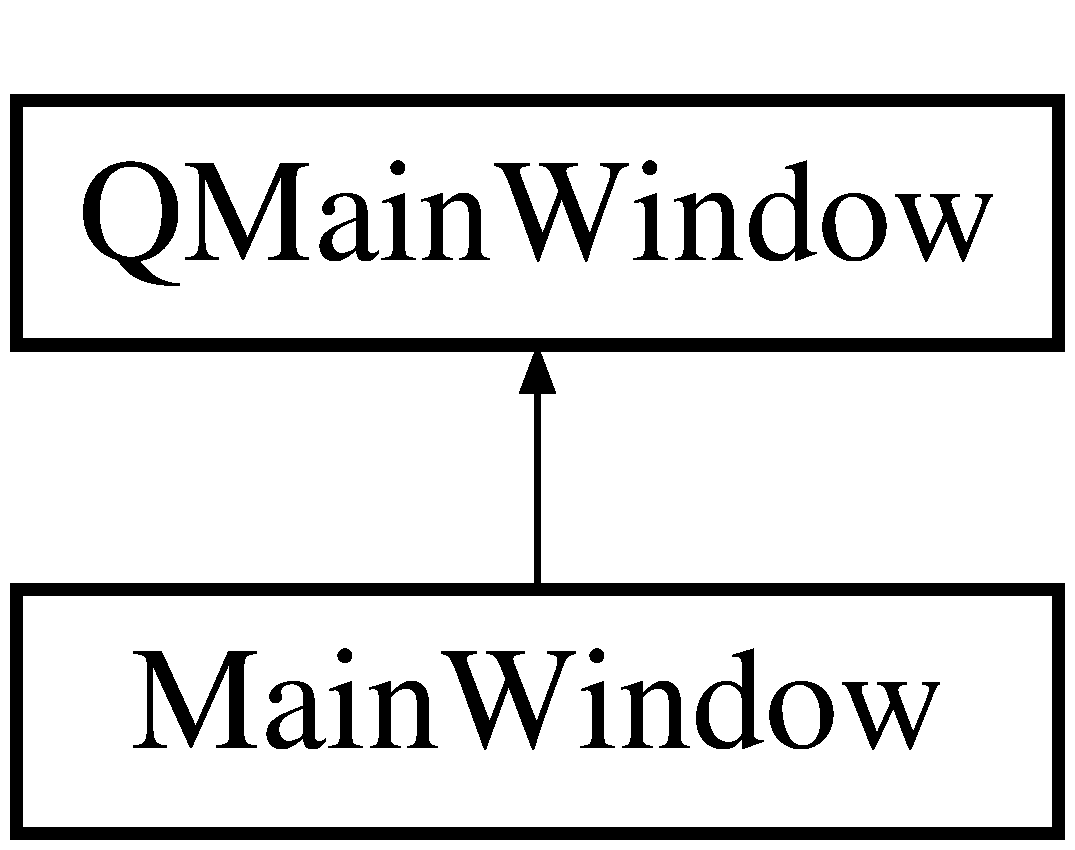
\includegraphics[height=2.000000cm]{class_main_window}
\end{center}
\end{figure}
\subsection*{Signals}
\begin{DoxyCompactItemize}
\item 
\hypertarget{class_main_window_a79ee89a481e69b71e4952b7adac270f7}{void {\bfseries start\+Audio} ()}\label{class_main_window_a79ee89a481e69b71e4952b7adac270f7}

\item 
\hypertarget{class_main_window_a08aaa1bf83576559bd4381a9eb88957d}{void {\bfseries end\+Audio} ()}\label{class_main_window_a08aaa1bf83576559bd4381a9eb88957d}

\item 
\hypertarget{class_main_window_aa29e66c3b8e0c48e0d6ba5df941c37ea}{void {\bfseries device\+Changed} (Q\+Audio\+Device\+Info devinfo)}\label{class_main_window_aa29e66c3b8e0c48e0d6ba5df941c37ea}

\item 
\hypertarget{class_main_window_accdf2b19b399a0c4e5edb079c45dfb4f}{void {\bfseries send\+Control\+String} (Q\+String data)}\label{class_main_window_accdf2b19b399a0c4e5edb079c45dfb4f}

\item 
\hypertarget{class_main_window_a9fab109300b5ff9a8c3a59f782a07d0b}{void {\bfseries end\+Broadcast} ()}\label{class_main_window_a9fab109300b5ff9a8c3a59f782a07d0b}

\end{DoxyCompactItemize}
\subsection*{Public Member Functions}
\begin{DoxyCompactItemize}
\item 
\hypertarget{class_main_window_a8b244be8b7b7db1b08de2a2acb9409db}{{\bfseries Main\+Window} (Q\+Widget $\ast$parent=0)}\label{class_main_window_a8b244be8b7b7db1b08de2a2acb9409db}

\end{DoxyCompactItemize}
\subsection*{Private Slots}
\begin{DoxyCompactItemize}
\item 
\hypertarget{class_main_window_afd714419be50b54076e7defa280ce0e3}{void {\bfseries get\+Device\+Info} ()}\label{class_main_window_afd714419be50b54076e7defa280ce0e3}

\item 
\hypertarget{class_main_window_a08231d6226a89db2eba0ebd94634a0c8}{void {\bfseries process\+Broadcast} (Q\+String address, Q\+String control\+String)}\label{class_main_window_a08231d6226a89db2eba0ebd94634a0c8}

\item 
\hypertarget{class_main_window_abf5188451c7c8934d2b083cc0cee6c89}{void {\bfseries on\+\_\+listen\+Button\+\_\+clicked} ()}\label{class_main_window_abf5188451c7c8934d2b083cc0cee6c89}

\item 
\hypertarget{class_main_window_a9fcfca6d7ffa439664532bfaea187614}{void {\bfseries on\+\_\+broadcast\+Button\+\_\+clicked} ()}\label{class_main_window_a9fcfca6d7ffa439664532bfaea187614}

\item 
\hypertarget{class_main_window_ac6fe47c1da6097f1e82f95a62df80ce4}{void {\bfseries on\+\_\+stop\+Listen\+Button\+\_\+clicked} ()}\label{class_main_window_ac6fe47c1da6097f1e82f95a62df80ce4}

\item 
\hypertarget{class_main_window_a9789c66a7bebb0e87ee9bac0f1d11b18}{void {\bfseries on\+\_\+end\+Broadcast\+Button\+\_\+clicked} ()}\label{class_main_window_a9789c66a7bebb0e87ee9bac0f1d11b18}

\item 
\hypertarget{class_main_window_abe3368d7caf1c748a2d76605ec2f054d}{void {\bfseries on\+\_\+output\+Volume\+Control\+\_\+slider\+Moved} (int position)}\label{class_main_window_abe3368d7caf1c748a2d76605ec2f054d}

\item 
\hypertarget{class_main_window_a396f4f5f9647db90598dae948d56ef70}{void {\bfseries on\+\_\+input\+Volume\+Control\+\_\+slider\+Moved} (int position)}\label{class_main_window_a396f4f5f9647db90598dae948d56ef70}

\item 
\hypertarget{class_main_window_a9f27c5371f7dab39063a41706c5efa09}{void {\bfseries on\+\_\+device\+Combo\+Box\+\_\+current\+Index\+Changed} (int index)}\label{class_main_window_a9f27c5371f7dab39063a41706c5efa09}

\end{DoxyCompactItemize}
\subsection*{Private Attributes}
\begin{DoxyCompactItemize}
\item 
\hypertarget{class_main_window_a35466a70ed47252a0191168126a352a5}{Ui\+::\+Main\+Window $\ast$ {\bfseries ui}}\label{class_main_window_a35466a70ed47252a0191168126a352a5}

\item 
\hypertarget{class_main_window_a5ff30e3e49a45f2b768cff8287c8cee3}{\hyperlink{class_client}{Client} $\ast$ {\bfseries client}}\label{class_main_window_a5ff30e3e49a45f2b768cff8287c8cee3}

\item 
\hypertarget{class_main_window_aca501db88230221cadf592104aa37ee5}{\hyperlink{class_server}{Server} $\ast$ {\bfseries server}}\label{class_main_window_aca501db88230221cadf592104aa37ee5}

\item 
\hypertarget{class_main_window_a9037ac1b7578485d6733a5d9a93ea04e}{\hyperlink{class_client_list}{Client\+List} $\ast$ {\bfseries clients}}\label{class_main_window_a9037ac1b7578485d6733a5d9a93ea04e}

\item 
\hypertarget{class_main_window_a7b2bc2ba82b635e3fe38c16228089a69}{Q\+Thread $\ast$ {\bfseries server\+Thread}}\label{class_main_window_a7b2bc2ba82b635e3fe38c16228089a69}

\item 
\hypertarget{class_main_window_a91a3d3c80f2654854f8879fcfbc55f97}{Q\+Thread $\ast$ {\bfseries client\+Thread}}\label{class_main_window_a91a3d3c80f2654854f8879fcfbc55f97}

\end{DoxyCompactItemize}


\subsection{Detailed Description}
The \hyperlink{class_main_window}{Main\+Window} class, view for the application. 

The documentation for this class was generated from the following files\+:\begin{DoxyCompactItemize}
\item 
soft336/mainwindow.\+h\item 
soft336/mainwindow.\+cpp\end{DoxyCompactItemize}

\hypertarget{class_server}{\section{Server Class Reference}
\label{class_server}\index{Server@{Server}}
}


The \hyperlink{class_server}{Server} class, responsible for reading from the audio device and sending across the network, and sending broadcast information.  




{\ttfamily \#include $<$server.\+h$>$}

Inheritance diagram for Server\+:\begin{figure}[H]
\begin{center}
\leavevmode
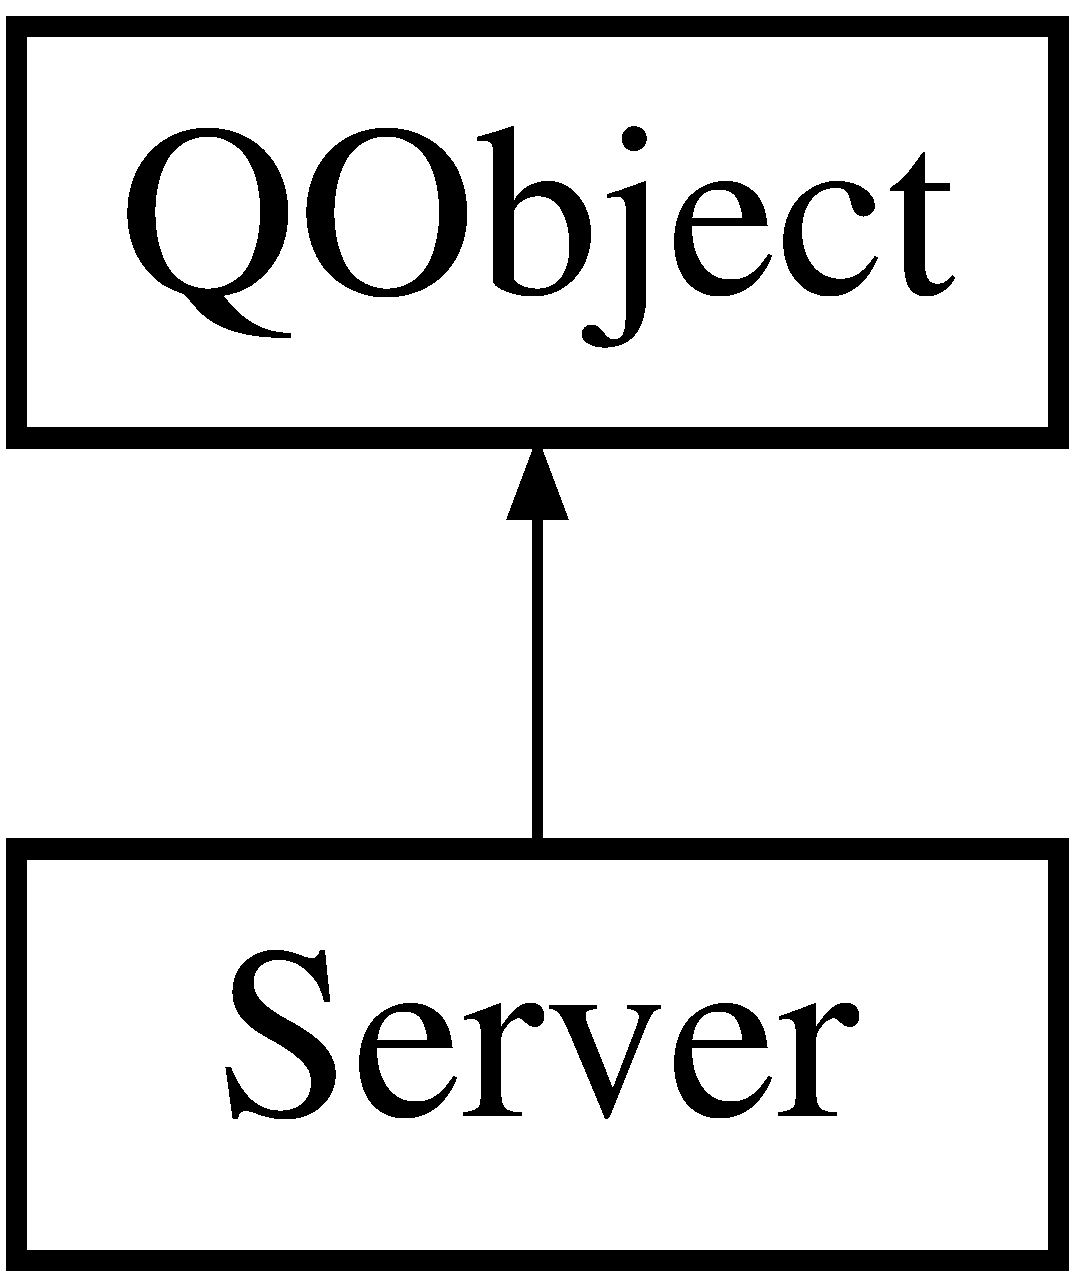
\includegraphics[height=2.000000cm]{class_server}
\end{center}
\end{figure}
\subsection*{Public Slots}
\begin{DoxyCompactItemize}
\item 
void \hyperlink{class_server_a47ec2f74efe239057a33fa20183f8417}{write\+Datagram} (Q\+Byte\+Array data)
\begin{DoxyCompactList}\small\item\em \hyperlink{class_server_a47ec2f74efe239057a33fa20183f8417}{Server\+::write\+Datagram} write audio datagram(s) to all clients (excluding this one). \end{DoxyCompactList}\item 
\hypertarget{class_server_aa2bc8edebbe7c55cda13e35969d288d8}{void \hyperlink{class_server_aa2bc8edebbe7c55cda13e35969d288d8}{start\+Audio\+Send} ()}\label{class_server_aa2bc8edebbe7c55cda13e35969d288d8}

\begin{DoxyCompactList}\small\item\em \hyperlink{class_server_aa2bc8edebbe7c55cda13e35969d288d8}{Server\+::start\+Audio\+Send} initiates the audio device. \end{DoxyCompactList}\item 
\hypertarget{class_server_a894e78a064ebbf6c0a82520941fc587b}{void \hyperlink{class_server_a894e78a064ebbf6c0a82520941fc587b}{end\+Audio\+Send} ()}\label{class_server_a894e78a064ebbf6c0a82520941fc587b}

\begin{DoxyCompactList}\small\item\em \hyperlink{class_server_a894e78a064ebbf6c0a82520941fc587b}{Server\+::end\+Audio\+Send} stops the audio device. \end{DoxyCompactList}\item 
void \hyperlink{class_server_a6754ec9f0275c85ea2e21047d2800b06}{change\+Device} (Q\+Audio\+Device\+Info devinfo)
\begin{DoxyCompactList}\small\item\em \hyperlink{class_server_a6754ec9f0275c85ea2e21047d2800b06}{Server\+::change\+Device} changes the audio device. \end{DoxyCompactList}\end{DoxyCompactItemize}
\subsection*{Public Member Functions}
\begin{DoxyCompactItemize}
\item 
\hyperlink{class_server_a5132484423532e71a8836c520f340e0a}{Server} (\hyperlink{class_client_list}{Client\+List} $\ast$clients, Q\+Object $\ast$parent=0)
\begin{DoxyCompactList}\small\item\em \hyperlink{class_server_a5132484423532e71a8836c520f340e0a}{Server\+::\+Server} default constructor for the server. \end{DoxyCompactList}\item 
void \hyperlink{class_server_a8dda22fb0d54f1ad3eb9c69017d98493}{set\+Volume} (float volume)
\begin{DoxyCompactList}\small\item\em \hyperlink{class_server_a8dda22fb0d54f1ad3eb9c69017d98493}{Server\+::set\+Volume} sets the volume of the input device. \end{DoxyCompactList}\end{DoxyCompactItemize}
\subsection*{Public Attributes}
\begin{DoxyCompactItemize}
\item 
\hypertarget{class_server_af1a9716febd17e14cce48a4ae2a0bce7}{\hyperlink{class_client_list}{Client\+List} $\ast$ {\bfseries client\+List}}\label{class_server_af1a9716febd17e14cce48a4ae2a0bce7}

\item 
\hypertarget{class_server_a23214ead7157ba34b1700434bf4ea8bd}{Q\+Host\+Address {\bfseries server\+I\+P}}\label{class_server_a23214ead7157ba34b1700434bf4ea8bd}

\end{DoxyCompactItemize}
\subsection*{Private Slots}
\begin{DoxyCompactItemize}
\item 
\hypertarget{class_server_a69da6d068b11feb5997dbfd6c8f863ac}{void \hyperlink{class_server_a69da6d068b11feb5997dbfd6c8f863ac}{send\+Update} ()}\label{class_server_a69da6d068b11feb5997dbfd6c8f863ac}

\begin{DoxyCompactList}\small\item\em \hyperlink{class_server_a69da6d068b11feb5997dbfd6c8f863ac}{Server\+::send\+Update} sends an update broadcast, informing clients of our status. \end{DoxyCompactList}\item 
void \hyperlink{class_server_a879b092399f867d8861e633192c10d47}{update\+Broadcast} (Q\+String data)
\begin{DoxyCompactList}\small\item\em \hyperlink{class_server_a879b092399f867d8861e633192c10d47}{Server\+::update\+Broadcast} updates the outgoing broadcast message. \end{DoxyCompactList}\end{DoxyCompactItemize}
\subsection*{Private Attributes}
\begin{DoxyCompactItemize}
\item 
\hypertarget{class_server_a66b3bdb5780364b9b13ce3836d23d30b}{Q\+Udp\+Socket $\ast$ {\bfseries socket}}\label{class_server_a66b3bdb5780364b9b13ce3836d23d30b}

\item 
\hypertarget{class_server_a9a123df402663d5cf77d37136a215660}{Q\+Timer $\ast$ {\bfseries broadcast\+Timer}}\label{class_server_a9a123df402663d5cf77d37136a215660}

\item 
\hypertarget{class_server_ae768ef05853969d0f7f0870b2e1b1d06}{\hyperlink{class_audio_input}{Audio\+Input} $\ast$ {\bfseries input}}\label{class_server_ae768ef05853969d0f7f0870b2e1b1d06}

\item 
\hypertarget{class_server_aaf9d54e01e90583f80efb6c63d15bae8}{Q\+Audio\+Device\+Info {\bfseries devinfo}}\label{class_server_aaf9d54e01e90583f80efb6c63d15bae8}

\item 
\hypertarget{class_server_a3ff13bf8f7dcaf334dd341f8b89907ce}{Q\+String {\bfseries broadcast\+Status}}\label{class_server_a3ff13bf8f7dcaf334dd341f8b89907ce}

\item 
\hypertarget{class_server_a5c32c8303cc0d59379af55769d678820}{Q\+String {\bfseries listening\+Status}}\label{class_server_a5c32c8303cc0d59379af55769d678820}

\end{DoxyCompactItemize}


\subsection{Detailed Description}
The \hyperlink{class_server}{Server} class, responsible for reading from the audio device and sending across the network, and sending broadcast information. 

\subsection{Constructor \& Destructor Documentation}
\hypertarget{class_server_a5132484423532e71a8836c520f340e0a}{\index{Server@{Server}!Server@{Server}}
\index{Server@{Server}!Server@{Server}}
\subsubsection[{Server}]{\setlength{\rightskip}{0pt plus 5cm}Server\+::\+Server (
\begin{DoxyParamCaption}
\item[{{\bf Client\+List} $\ast$}]{clients, }
\item[{Q\+Object $\ast$}]{parent = {\ttfamily 0}}
\end{DoxyParamCaption}
)\hspace{0.3cm}{\ttfamily [explicit]}}}\label{class_server_a5132484423532e71a8836c520f340e0a}


\hyperlink{class_server_a5132484423532e71a8836c520f340e0a}{Server\+::\+Server} default constructor for the server. 


\begin{DoxyParams}{Parameters}
{\em clients} & pointer to the clients object we will read from when sending to clients. \\
\hline
{\em parent} & the parent object. \\
\hline
\end{DoxyParams}


\subsection{Member Function Documentation}
\hypertarget{class_server_a6754ec9f0275c85ea2e21047d2800b06}{\index{Server@{Server}!change\+Device@{change\+Device}}
\index{change\+Device@{change\+Device}!Server@{Server}}
\subsubsection[{change\+Device}]{\setlength{\rightskip}{0pt plus 5cm}void Server\+::change\+Device (
\begin{DoxyParamCaption}
\item[{Q\+Audio\+Device\+Info}]{devinfo}
\end{DoxyParamCaption}
)\hspace{0.3cm}{\ttfamily [slot]}}}\label{class_server_a6754ec9f0275c85ea2e21047d2800b06}


\hyperlink{class_server_a6754ec9f0275c85ea2e21047d2800b06}{Server\+::change\+Device} changes the audio device. 


\begin{DoxyParams}{Parameters}
{\em devinfo} & the audio device to change too. \\
\hline
\end{DoxyParams}
\hypertarget{class_server_a8dda22fb0d54f1ad3eb9c69017d98493}{\index{Server@{Server}!set\+Volume@{set\+Volume}}
\index{set\+Volume@{set\+Volume}!Server@{Server}}
\subsubsection[{set\+Volume}]{\setlength{\rightskip}{0pt plus 5cm}void Server\+::set\+Volume (
\begin{DoxyParamCaption}
\item[{float}]{volume}
\end{DoxyParamCaption}
)}}\label{class_server_a8dda22fb0d54f1ad3eb9c69017d98493}


\hyperlink{class_server_a8dda22fb0d54f1ad3eb9c69017d98493}{Server\+::set\+Volume} sets the volume of the input device. 


\begin{DoxyParams}{Parameters}
{\em volume} & the audio to set. \\
\hline
\end{DoxyParams}
\hypertarget{class_server_a879b092399f867d8861e633192c10d47}{\index{Server@{Server}!update\+Broadcast@{update\+Broadcast}}
\index{update\+Broadcast@{update\+Broadcast}!Server@{Server}}
\subsubsection[{update\+Broadcast}]{\setlength{\rightskip}{0pt plus 5cm}void Server\+::update\+Broadcast (
\begin{DoxyParamCaption}
\item[{Q\+String}]{data}
\end{DoxyParamCaption}
)\hspace{0.3cm}{\ttfamily [private]}, {\ttfamily [slot]}}}\label{class_server_a879b092399f867d8861e633192c10d47}


\hyperlink{class_server_a879b092399f867d8861e633192c10d47}{Server\+::update\+Broadcast} updates the outgoing broadcast message. 


\begin{DoxyParams}{Parameters}
{\em data} & string containing broadcast status update. \\
\hline
\end{DoxyParams}
\hypertarget{class_server_a47ec2f74efe239057a33fa20183f8417}{\index{Server@{Server}!write\+Datagram@{write\+Datagram}}
\index{write\+Datagram@{write\+Datagram}!Server@{Server}}
\subsubsection[{write\+Datagram}]{\setlength{\rightskip}{0pt plus 5cm}void Server\+::write\+Datagram (
\begin{DoxyParamCaption}
\item[{Q\+Byte\+Array}]{data}
\end{DoxyParamCaption}
)\hspace{0.3cm}{\ttfamily [slot]}}}\label{class_server_a47ec2f74efe239057a33fa20183f8417}


\hyperlink{class_server_a47ec2f74efe239057a33fa20183f8417}{Server\+::write\+Datagram} write audio datagram(s) to all clients (excluding this one). 


\begin{DoxyParams}{Parameters}
{\em data} & audio data to send. \\
\hline
\end{DoxyParams}


The documentation for this class was generated from the following files\+:\begin{DoxyCompactItemize}
\item 
soft336/server.\+h\item 
soft336/server.\+cpp\end{DoxyCompactItemize}

%--- End generated contents ---

% Index
\newpage
\phantomsection
\addcontentsline{toc}{chapter}{Index}
\printindex

\end{document}
